%!TEX root = ../assignment1.tex

\section{Findings Of Phase 2}

\subsection{Overview Of Data}
In Phase 2, 10 case studies are given on how projects failed in Victoria Australia. The cases are government-related information communication and technology projects. The author\parencite{case_study} provides well-structured anatomy of projects where issues are discussed in depth by topics. Additionally, some recommendations are given by the author, some of which is responded by the project owners.

\subsection{Gaps and Solutions}
Using the same method, we collect gaps and possible solutions(proposals) for further evaluation. There are 54 sections of gaps reflecting 54 proposals to 10 case studies, some of them are duplicated. The author uses no mathematical model to prioritize gaps, a baseline value of $1$ is also used to all the proposals, according to the predefined methodology.

The collected data are tagged with the same four themes: control, process, people and structure. Here are some samples under each theme.

\subsubsection{Samples: Control}
% id 21
In case 4, the author argues that the longer planning that spans in time, the more risk of redesigned. Ultimately, the project will be likely to fail due to this uncertainty of change. Project leaders should plan to fund well with top management support in the initial phase. As change happens at any time, if the project cycle is too long, the project will be more likely to require more funding. Correspondingly, the uncertainty of the project increases with time, and the initial design and costing plan are very likely to need to change over time, so the risk of project failure increases.


% id 2
In case 1, it is the rushing to meet deadlines that fails to deliver design goals. For cover-up, benefits are altered to please the government. Project managers should define the measurement of deliverables and change accordingly. A good case plan is the foundation of a project's success. If the case plan is just made to win the government support without respecting the facts, the result of project failure is foreseeable. In this case, many of benefits are unmeasurable but they are still written into the plan to please the government. Its failure is unavoidable.

\subsubsection{Samples: Process}
% id 26
Poor user training and post-implementation support result in bad experience among users. Better user training and support should be designed and implemented in the early stage of project planning. In case 5, even the project (CRIS) has been delivered to the end-users in July 2008, because of the lack of necessary training and the poor system support services, the feature change request from the user cannot get a proper response in time, which results in pretty low user satisfaction of the system.

% 30
The training cost is not included in the planning process. It is suggested to consider training in cost planning. In case 6, due to lack of adequate up-front planning, the project plan didn't include the expense for Ultranet coaches and the cost for school professional development day. Thus it caused a funding problem around \$23 million. A comprehensive plan is the cornerstone of the project's success, to avoid a funding gap, IT projects should be handled with care when reviewing funding plans.

\subsubsection{Samples: People}
% 34
Failing to detect risks of vendor results in bad contract deals. Vendor performance should be reviewed by a third party in planning. In case 7, even DOJ has made various efforts to address vendor performance issues, the vendor is still frequently failing to meet the promised timeline. In September 2008, the owner of the vendor changed, and DOJ had to renegotiate the contract with the new owner of the vendor. Due to fearing that the new owner would abandon the contract, DOJ had to make concessions on the liability for delay and the indemnity clause. This fully demonstrates the importance of an objective assessment of the supplier's performance capabilities. It is recommended that the tenderer should hire an independent, qualified third-party agency to evaluate the vendor's capabilities and historical performance.


% 37
Projects fail and lead to an alternative solution when requirements are not communicated precisely. It is important to understand the requirements and define the deliverables that the project manager and the end-user agree on.

According to the Supreme Court of Australia, ICMS’s case management system (CourtView) fails to meet the court’s needs. The Supreme Court has ultimately resolved to pilot its own system to provide case management. ICMS is a typical case which is developed by the client and vendor. The end user did not get an opportunity to participate in their opinion before the system is shipped to them. Systems developed in this way are very likely to cause dissatisfaction to end users. After all, most of the time, the people who pay (the customers or clients) are not the people who use the system. Not surprisingly, the Supreme Court finally chose to fund the development of the system it needed, spending only a small amount of money and getting a good satisfaction.

\subsubsection{Samples: Structure}
% 4
The vacancy of a project leader results in management chaos. It is important to have a project leader. Unfortunately, they appointed two project manager in case 1, one is a business project manager, the other is a technical project manager. Since none of them is authoritative, neither person is responsible for the overall result of the project. To make matters worse, after-the-fact investigations have shown that both project managers are lack experience in managing large IT projects. A qualified, authoritative is irreplaceable for such projects.

% 19
The organization structure stops from making timely funding to implement the project. A better organization is advised. There are uncertainties in any IT project, and good organizational and funding plans can help overcome these uncertainties. The VicRoads project did not receive follow-up development funds, as a result, the development team has basically been disbanded, and the project prospects are not good. VicRoads has already spent \$52 million in past years, it will be a huge waste to Australia government. 


\subsection{Evaluation Of Solutions}
To select the solutions out of all the proposals, we do the same evaluation steps as shown in \ref{section:evaluation}.

With the defined method, we tag all our research contexts as $C_{1}, C_{2}, \ldots, C_{10}$. We assume all the solutions from the 10 case studies are of equal importance, given the fact that there is no math model used in Phase 2. Therefore, we pad the cross-contextual coefficient with a baseline value of 1 to all the $\mathit{k_{C_{i},j}}$ in formula \ref{brief}. So formula \ref{final} can be simplified as 

\begin{equation}
g_{C_{i},j} = l_{C_{i},j} = |P_{C_{i,j}}| |R_{C_{i,j}}|
\label{formula:p2}
\end{equation}

With the updated formula \ref{formula:p2}, we calculate the global influence score for each proposal. Here is a visualization of the scores of all the proposals in Phase 2.

In the plot, there are 3 groups: the leading group of 3 proposals, the group of majority and the trailing group.

\begin{figure}[ht]
\centering
\resizebox{\columnwidth}{!}{%
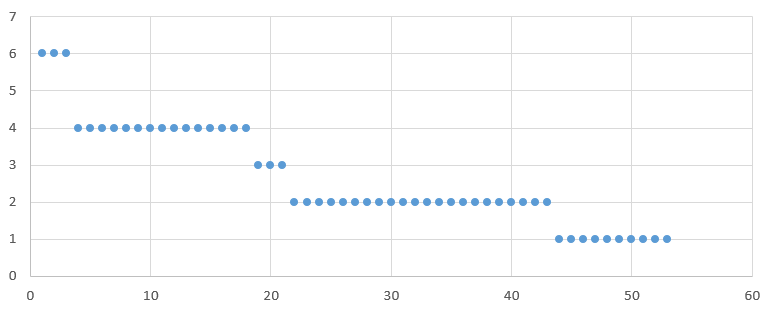
\includegraphics{global_influence_score_p2.png}
}
\end{figure}
\subsection{Result Of Evaluation}
We calculate the average score using the same way($\bar{g}=1.37$), which truncates the trailing group. The selected proposals are shown as follows.

\begin{table}[ht]
\caption{Solution List Of Phase 2}
\begin{adjustbox}{width=1\textwidth}
\csvautotabular{tables/solutions_p2.csv}
\end{adjustbox}
\label{tab:solution2}
\end{table}
